%!TEX root =../mapp-hsc17-game-book.tex
% ^ leave for LaTeXTools build functionality

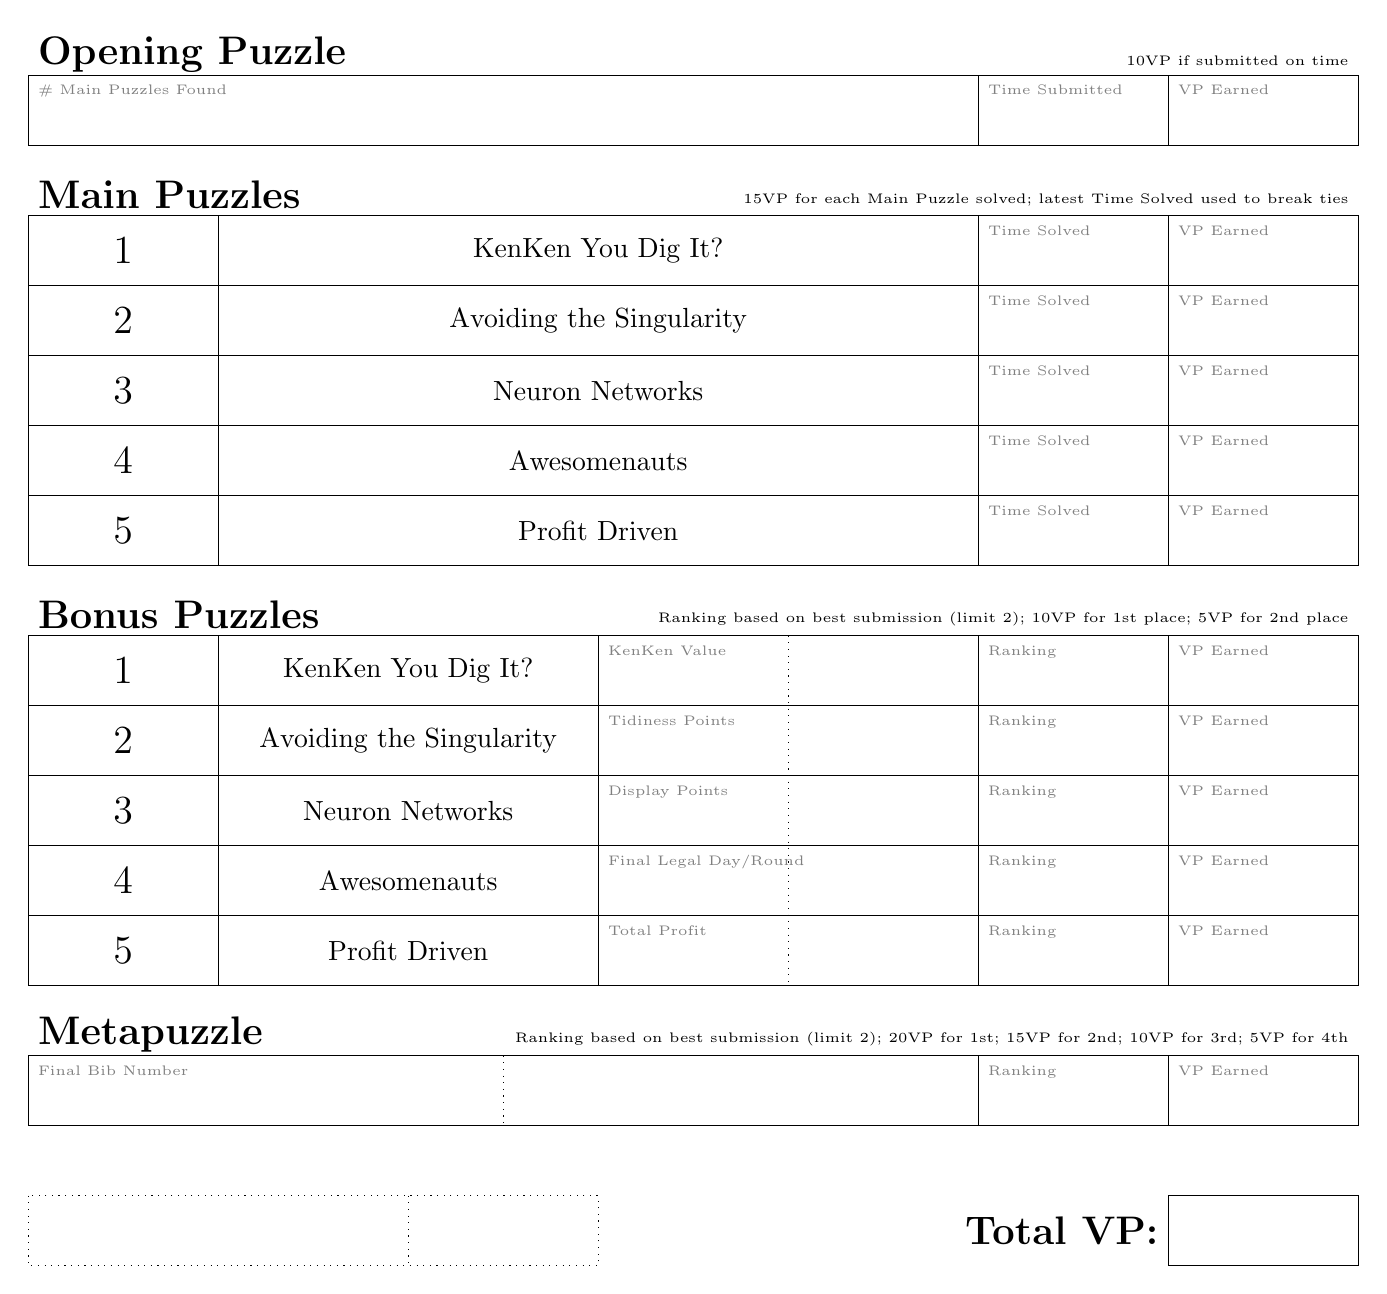
\begin{tikzpicture}[x=0.95in,y=-0.35in]
  % \draw (0,0) rectangle +(6,1);
  % \draw (1,0) -- +(0,1);

  \node[anchor=west] at (0,1.7) {\Large\bf Opening Puzzle};
  \draw (0,2) rectangle +(7,1);
  \draw (5,2) -- +(0,1);
  \draw (6,2) -- +(0,1);
  \node[color=gray,anchor=north west] at (0,2)
    {\tiny \# Main Puzzles Found};
  \node[color=gray,anchor=north west] at (5,2)
    {\tiny Time Submitted};
  \node[color=gray,anchor=north west] at (6,2)
    {\tiny VP Earned};
  \node[anchor=south east] at (7,2)
    {\tiny 10VP if submitted on time};

  \node[anchor=west] at (0,3.7) {\Large\bf Main Puzzles};
  \draw (0,4) rectangle +(7,5);
  \draw (0,5) -- +(7,0);
  \draw (0,6) -- +(7,0);
  \draw (0,7) -- +(7,0);
  \draw (0,8) -- +(7,0);
  \draw (1,4) -- +(0,5);
  \draw (5,4) -- +(0,5);
  \draw (6,4) -- +(0,5);
  \node at (0.5,4.5) {\Large 1};
  \node at (0.5,5.5) {\Large 2};
  \node at (0.5,6.5) {\Large 3};
  \node at (0.5,7.5) {\Large 4};
  \node at (0.5,8.5) {\Large 5};
  \node at (3,4.5) {KenKen You Dig It?};
  \node at (3,5.5) {Avoiding the Singularity};
  \node at (3,6.5) {Neuron Networks};
  \node at (3,7.5) {Awesomenauts};
  \node at (3,8.5) {Profit Driven};
  \node[color=gray,anchor=north west] at (5,4)
    {\tiny Time Solved};
  \node[color=gray,anchor=north west] at (5,5)
    {\tiny Time Solved};
  \node[color=gray,anchor=north west] at (5,6)
    {\tiny Time Solved};
  \node[color=gray,anchor=north west] at (5,7)
    {\tiny Time Solved};
  \node[color=gray,anchor=north west] at (5,8)
    {\tiny Time Solved};
  \node[color=gray,anchor=north west] at (6,4)
    {\tiny VP Earned};
  \node[color=gray,anchor=north west] at (6,5)
    {\tiny VP Earned};
  \node[color=gray,anchor=north west] at (6,6)
    {\tiny VP Earned};
  \node[color=gray,anchor=north west] at (6,7)
    {\tiny VP Earned};
  \node[color=gray,anchor=north west] at (6,8)
    {\tiny VP Earned};
  \node[anchor=south east] at (7,4)
    {\tiny 15VP for each Main Puzzle solved; latest Time Solved used to break ties};

  \node[anchor=west] at (0,9.7) {\Large\bf Bonus Puzzles};
  \draw (0,10) rectangle +(7,5);
  \draw (0,11) -- +(7,0);
  \draw (0,12) -- +(7,0);
  \draw (0,13) -- +(7,0);
  \draw (0,14) -- +(7,0);
  \draw (1,10) -- +(0,5);
  \draw (3,10) -- +(0,5);
  \draw[dotted] (4,10) -- +(0,5);
  \draw (5,10) -- +(0,5);
  \draw (6,10) -- +(0,5);
  \node at (0.5,10.5) {\Large 1};
  \node at (0.5,11.5) {\Large 2};
  \node at (0.5,12.5) {\Large 3};
  \node at (0.5,13.5) {\Large 4};
  \node at (0.5,14.5) {\Large 5};
  \node at (2,10.5) {KenKen You Dig It?};
  \node at (2,11.5) {Avoiding the Singularity};
  \node at (2,12.5) {Neuron Networks};
  \node at (2,13.5) {Awesomenauts};
  \node at (2,14.5) {Profit Driven};
  \node[color=gray,anchor=north west] at (3,10)
    {\tiny KenKen Value};
  \node[color=gray,anchor=north west] at (3,11)
    {\tiny Tidiness Points};
  \node[color=gray,anchor=north west] at (3,12)
    {\tiny Display Points};
  \node[color=gray,anchor=north west] at (3,13)
    {\tiny Final Legal Day/Round};
  \node[color=gray,anchor=north west] at (3,14)
    {\tiny Total Profit};
  \node[color=gray,anchor=north west] at (5,10)
    {\tiny Ranking};
  \node[color=gray,anchor=north west] at (5,11)
    {\tiny Ranking};
  \node[color=gray,anchor=north west] at (5,12)
    {\tiny Ranking};
  \node[color=gray,anchor=north west] at (5,13)
    {\tiny Ranking};
  \node[color=gray,anchor=north west] at (5,14)
    {\tiny Ranking};
  \node[color=gray,anchor=north west] at (6,10)
    {\tiny VP Earned};
  \node[color=gray,anchor=north west] at (6,11)
    {\tiny VP Earned};
  \node[color=gray,anchor=north west] at (6,12)
    {\tiny VP Earned};
  \node[color=gray,anchor=north west] at (6,13)
    {\tiny VP Earned};
  \node[color=gray,anchor=north west] at (6,14)
    {\tiny VP Earned};
  \node[anchor=south east] at (7,10)
    {\tiny Ranking based on best submission (limit 2); 10VP for 1st place;
      5VP for 2nd place};

  \node[anchor=west] at (0,15.7) {\Large\bf Metapuzzle};
  \draw (0,16) rectangle +(7,1);
  \draw[dotted] (2.5,16) -- +(0,1);
  \draw (5,16) -- +(0,1);
  \draw (6,16) -- +(0,1);
  \node[color=gray,anchor=north west] at (0,16)
    {\tiny Final Bib Number};
  \node[color=gray,anchor=north west] at (5,16)
    {\tiny Ranking};
  \node[color=gray,anchor=north west] at (6,16)
    {\tiny VP Earned};
  \node[anchor=south east] at (7,16)
    {\tiny Ranking based on best submission (limit 2);
      20VP for 1st; 15VP for 2nd; 10VP for 3rd; 5VP for 4th};

  \draw[dotted] (0,18) rectangle +(3,1);
  \draw[dotted] (2,18) -- +(0,1);

  \node[anchor=east] at (6,18.5) {\Large\bf Total VP:};
  \draw (6,18) rectangle +(1,1);
\end{tikzpicture}

\vspace{1em}

{\noindent\LARGE Team Number: \underline{\hspace{0.5in}}
School Name: \underline{\hspace{3in}}}

{\footnotesize\noindent
Game Control and your team each have a copy of this scoresheet. You must
bring your team's copy to Game Control to submit solutions.}


%%% Local Variables:
%%% mode: latex
%%% TeX-master: "../mapp-hsc17-game-book"
%%% End:
